\documentclass[tikz,border=6pt]{standalone}
\usepackage[T1]{fontenc}
\usepackage{lmodern}
\usepackage{amsmath,amssymb}
\usetikzlibrary{positioning,arrows.meta,fit,calc}
% Design of koblitz-n83-indexbuild-20261020 (frozen protocol.json and schedule.json). Not a result.
\begin{document}
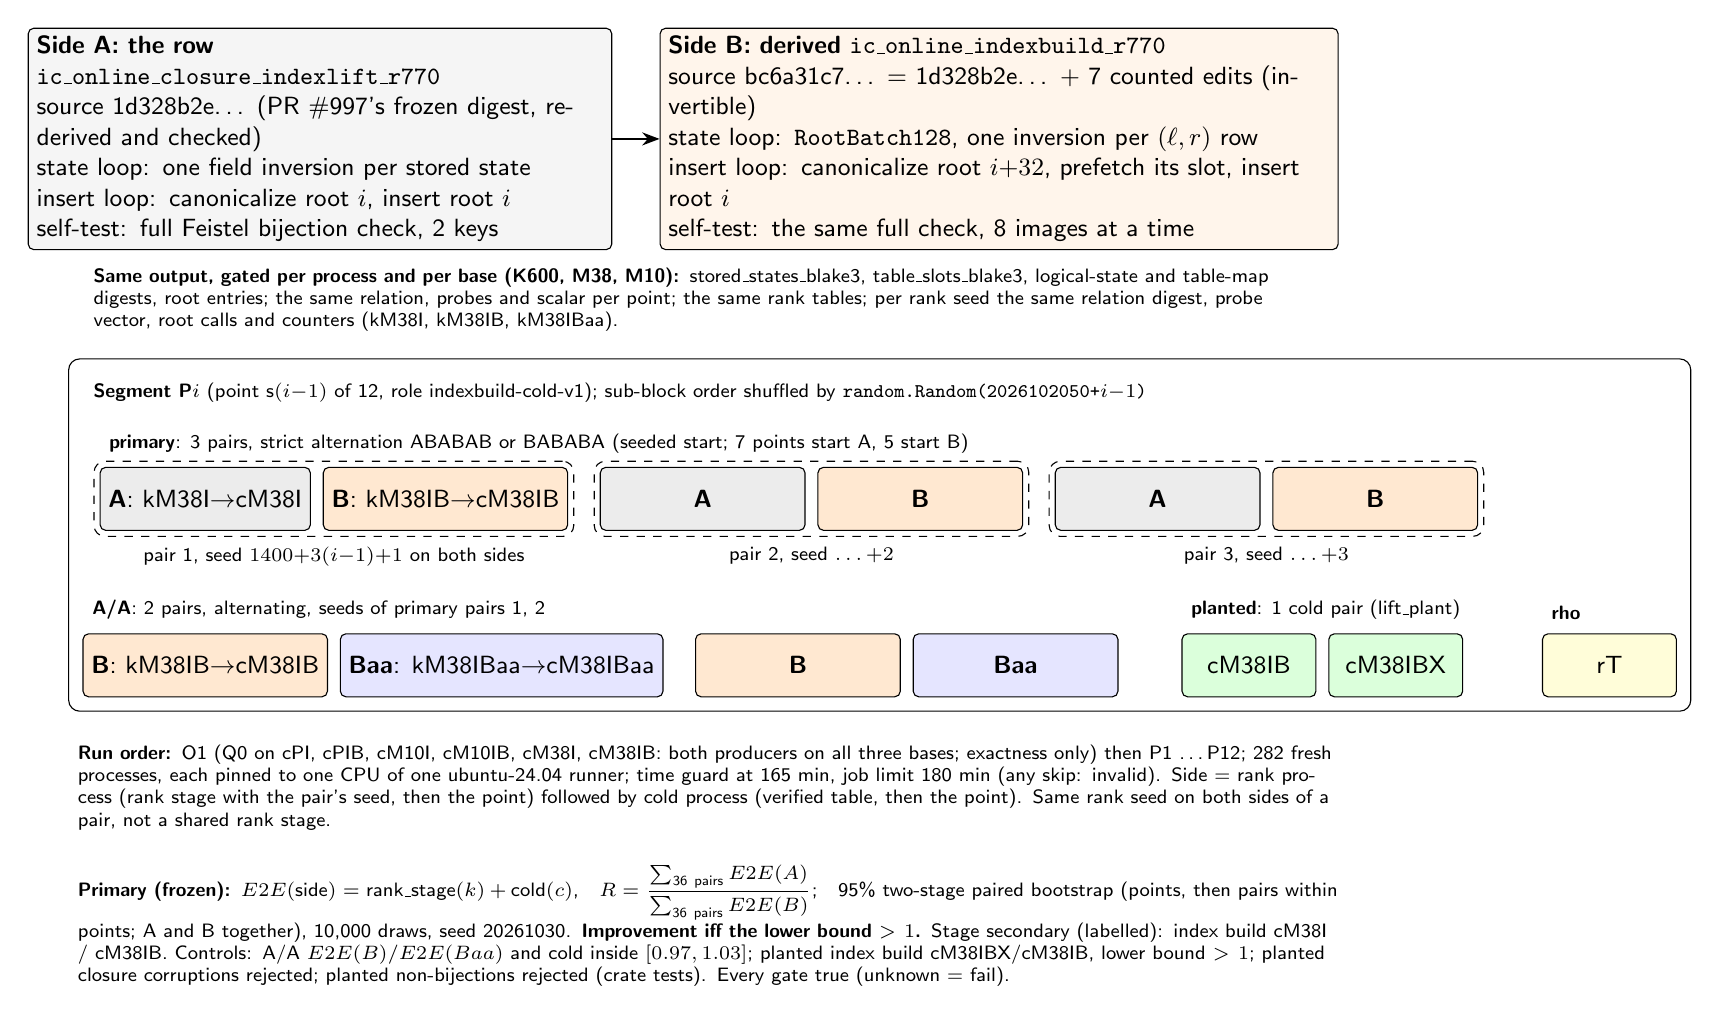
\begin{tikzpicture}[
  font=\sffamily\small,
  box/.style={draw, rounded corners=2pt, align=center, minimum height=8mm, inner sep=3pt},
  sa/.style={box, fill=gray!15, minimum width=26mm},
  sb/.style={box, fill=orange!18, minimum width=26mm},
  sc/.style={box, fill=blue!10, minimum width=26mm},
  sx/.style={box, fill=green!14, minimum width=17mm},
  arr/.style={-{Stealth[length=2.2mm]}, thick},
  note/.style={align=left, font=\sffamily\scriptsize}
]
% producers
\node[box, fill=gray!8, text width=72mm, align=left] (pa) {\textbf{Side A: the row} \texttt{ic\_online\_closure\_indexlift\_r770}\\
source 1d328b2e\ldots\ (PR \#997's frozen digest, re-derived and checked)\\
state loop: one field inversion per stored state\\
insert loop: canonicalize root $i$, insert root $i$\\
self-test: full Feistel bijection check, 2 keys};
\node[box, fill=orange!8, text width=84mm, align=left, right=6mm of pa] (pb) {\textbf{Side B: derived} \texttt{ic\_online\_indexbuild\_r770}\\
source bc6a31c7\ldots\ = 1d328b2e\ldots\ + 7 counted edits (invertible)\\
state loop: \texttt{RootBatch128}, one inversion per $(\ell,r)$ row\\
insert loop: canonicalize root $i{+}32$, prefetch its slot, insert root $i$\\
self-test: the same full check, 8 images at a time};
\draw[arr] (pa.east) -- (pb.west);
\node[note, below=1mm of pb.south, anchor=north, text width=150mm, xshift=-40mm] (same) {\textbf{Same output, gated per process and per base (K600, M38, M10):} stored\_states\_blake3, table\_slots\_blake3, logical-state and table-map digests, root entries; the same relation, probes and scalar per point; the same rank tables; per rank seed the same relation digest, probe vector, root calls and counters (kM38I, kM38IB, kM38IBaa).};
% one point segment
\node[note, below=4mm of same.south west, anchor=north west] (ptitle) {\textbf{Segment P$i$} (point s$(i{-}1)$ of 12, role indexbuild-cold-v1); sub-block order shuffled by \texttt{random.Random(2026102050+$i{-}1$)}};
% primary block
\node[sa, below=7mm of ptitle.south west, anchor=north west, xshift=2mm] (a1) {\textbf{A}: kM38I$\to$cM38I};
\node[sb, right=1.5mm of a1] (b1) {\textbf{B}: kM38IB$\to$cM38IB};
\node[sa, right=4mm of b1] (a2) {\textbf{A}};
\node[sb, right=1.5mm of a2] (b2) {\textbf{B}};
\node[sa, right=4mm of b2] (a3) {\textbf{A}};
\node[sb, right=1.5mm of a3] (b3) {\textbf{B}};
\node[draw, dashed, rounded corners, fit=(a1) (b1), inner sep=2pt, label={[note]below:pair 1, seed $1400{+}3(i{-}1){+}1$ on both sides}] {};
\node[draw, dashed, rounded corners, fit=(a2) (b2), inner sep=2pt, label={[note]below:pair 2, seed $\ldots{+}2$}] {};
\node[draw, dashed, rounded corners, fit=(a3) (b3), inner sep=2pt, label={[note]below:pair 3, seed $\ldots{+}3$}] {};
\node[note, above=0.5mm of a1.north west, anchor=south west] {\textbf{primary}: 3 pairs, strict alternation ABABAB or BABABA (seeded start; 7 points start A, 5 start B)};
% aa block
\node[sb, below=13mm of a1] (aa1) {\textbf{B}: kM38IB$\to$cM38IB};
\node[sc, right=1.5mm of aa1] (aa2) {\textbf{Baa}: kM38IBaa$\to$cM38IBaa};
\node[sb, right=4mm of aa2] (aa3) {\textbf{B}};
\node[sc, right=1.5mm of aa3] (aa4) {\textbf{Baa}};
\node[note, above=0.5mm of aa1.north west, anchor=south west] {\textbf{A/A}: 2 pairs, alternating, seeds of primary pairs 1, 2};
% planted
\node[sx, right=8mm of aa4] (p1) {cM38IB};
\node[sx, right=1.5mm of p1] (p2) {cM38IBX};
\node[note, above=0.5mm of p1.north west, anchor=south west] {\textbf{planted}: 1 cold pair (lift\_plant)};
\node[sx, right=10mm of p2, fill=yellow!15] (rt) {rT};
\node[note, above=0.5mm of rt.north west, anchor=south west] {\textbf{rho}};
\node[draw, rounded corners, fit=(ptitle) (a1) (b3) (aa1) (rt), inner sep=5pt] (seg) {};
\node[note, below=3mm of seg.south west, anchor=north west, text width=160mm] (order) {\textbf{Run order:} O1 (Q0 on cPI, cPIB, cM10I, cM10IB, cM38I, cM38IB: both producers on all three bases; exactness only) then P1 \ldots P12; 282 fresh processes, each pinned to one CPU of one ubuntu-24.04 runner; time guard at 165 min, job limit 180 min (any skip: invalid).
Side = rank process (rank stage with the pair's seed, then the point) followed by cold process (verified table, then the point). Same rank seed on both sides of a pair, not a shared rank stage.};
\node[note, below=2mm of order.south west, anchor=north west, text width=160mm] (prim) {\textbf{Primary (frozen):}
$E2E(\text{side}) = \text{rank\_stage}(k) + \text{cold}(c)$,\quad
$R=\dfrac{\sum_{\text{36 pairs}} E2E(A)}{\sum_{\text{36 pairs}} E2E(B)}$;\quad
95\% two-stage paired bootstrap (points, then pairs within points; A and B together), 10{,}000 draws, seed 20261030.
\textbf{Improvement iff the lower bound $>1$.} Stage secondary (labelled): index build cM38I / cM38IB. Controls: A/A $E2E(B)/E2E(Baa)$ and cold inside $[0.97,1.03]$; planted index build cM38IBX/cM38IB, lower bound $>1$; planted closure corruptions rejected; planted non-bijections rejected (crate tests). Every gate true (unknown = fail).};
\end{tikzpicture}
\end{document}
